\documentclass[12pt,a4paper]{article}

%------------------------------------------------
% PACKAGES
%------------------------------------------------
\usepackage[utf8]{inputenc}
\usepackage[T1]{fontenc}
\usepackage{geometry}
\usepackage{graphicx}
\usepackage{booktabs}
\usepackage{array}
\usepackage{longtable}
\usepackage{float}
\usepackage{setspace}
\usepackage{titlesec}
\usepackage{hyperref}

\geometry{margin=2.5cm}
\setstretch{1.5}

%------------------------------------------------
% TITLE
%------------------------------------------------
\title{
\textbf{Phase 1: Problem Definition} \\
Comparative Analysis of Machine Learning Architectures \\
for Satellite-Based Surface Monitoring \\
\vspace{0.5cm}
Case Study: Armero, Colombia
}

\author{
Mar\'ia Lizarazo, Valeria Herrera, Juan Tellez, Andr\'e Landinez, Santiago Mesa \\
Pontificia Universidad Javeriana
}

\date{\today}

%------------------------------------------------
% DOCUMENT
%------------------------------------------------
\begin{document}

\maketitle
\tableofcontents
\newpage

%------------------------------------------------
\section{Introduction}
%------------------------------------------------

The municipality of Armero, located in the department of Tolima, Colombia, was the site of one of the deadliest volcanic disasters in Latin America. On November 13, 1985, the eruption of the Nevado del Ruiz volcano generated lahars that buried much of the town, causing approximately 25,000 casualties and severe environmental transformation of the surrounding landscape.

This project aims to analyze the current land surface cover of the Armero region using Sentinel-2 multispectral satellite imagery and supervised machine learning techniques. Through spectral analysis and classification models, the study seeks to identify and quantify different land cover classes such as vegetation, croplands, bare soil, and urban areas.

The project follows a GeoAI workflow in which satellite spectral information is transformed into structured datasets for machine learning-based land cover prediction, independent of traditional GIS software.

%------------------------------------------------
\section{Event Selection}
%------------------------------------------------

The selected case study corresponds to the Armero region in Tolima, Colombia, affected historically by the Nevado del Ruiz volcanic eruption on November 13, 1985.

\subsection{Reasons for Selection}

\begin{itemize}
    \item Historical and environmental relevance: one of the worst volcanic disasters in Latin American history.
    \item Presence of heterogeneous land cover types: vegetation, croplands, bare soil, and urban zones.
    \item Availability of cloud-free Sentinel-2 L2A imagery.
    \item Suitable spectral diversity for supervised classification tasks.
\end{itemize}

The analysis focuses on identifying present-day surface conditions and understanding the spatial distribution of land cover categories within the study area.

%------------------------------------------------
\section{Study Area}
%------------------------------------------------

The Region of Interest (ROI) is centered on the former municipality of Armero, Tolima, Colombia, now known as Armero Guayabal.

\subsection{ROI Coordinates}

\begin{table}[H]
\centering
\begin{tabular}{|m{5cm}|m{7cm}|}
\hline
\textbf{Parameter} & \textbf{Value} \\
\hline
Minimum Longitude & $-74.97345^\circ$ W \\
\hline
Maximum Longitude & $-74.787712^\circ$ W \\
\hline
Minimum Latitude & $4.943197^\circ$ N \\
\hline
Maximum Latitude & $5.117959^\circ$ N \\
\hline
Approximate Center & $5.03^\circ$ N, $-74.88^\circ$ W \\
\hline
Total Area & 402.70 km$^2$ \\
\hline
\end{tabular}
\caption{ROI coordinates obtained from Copernicus Browser}
\end{table}

\subsection{Study Area Characteristics}

The selected ROI was drawn using the Copernicus Browser polygon tool and contains a diverse range of land cover types:

\begin{itemize}
    \item Agricultural areas and croplands in the flat zones of the Magdalena River valley
    \item Natural vegetation and forest patches on hillsides
    \item Bare soil and exposed terrain
    \item Small urban areas corresponding to Armero Guayabal
\end{itemize}

This diversity of spectral responses makes the region suitable for machine learning classification experiments.

\begin{figure}[H]
\centering

\includegraphics[width=0.85\textwidth]{roi_map.png}
\caption{Region of Interest (ROI) delimited over OpenStreetMap. The yellow rectangle covers approximately 402.70~km$^2$ centered on Armero Guayabal, Tolima, Colombia.}
\label{fig:roi}
\end{figure}

%------------------------------------------------
\section{Satellite Imagery Metadata}
%------------------------------------------------

The project uses multispectral imagery from the Sentinel-2 mission developed by the Copernicus Programme (ESA).

\subsection{Selected Satellite Product}

\begin{table}[H]
\centering
\begin{tabular}{|m{5cm}|m{8cm}|}
\hline
\textbf{Attribute} & \textbf{Value} \\
\hline
Product Name & S2A\_MSIL2A\_20240815T152651\_N0511\_R025\_T18NWL \\
\hline
Acquisition Date & August 15, 2024 \\
\hline
Sensing Time & 15:26:51 UTC \\
\hline
Processing Level & Level-2A (Bottom of Atmosphere) \\
\hline
Tile & T18NWL \\
\hline
Cloud Coverage & 15\% \\
\hline
Satellite & Sentinel-2A \\
\hline
Sensor & MSI (Multispectral Instrument) \\
\hline
Coordinate System & WGS84 / UTM Zone 18N (EPSG:32618) \\
\hline
Image Format & GeoTIFF (.tif) \\
\hline
\end{tabular}
\caption{Sentinel-2 product metadata}
\end{table}

\begin{figure}[H]
\centering
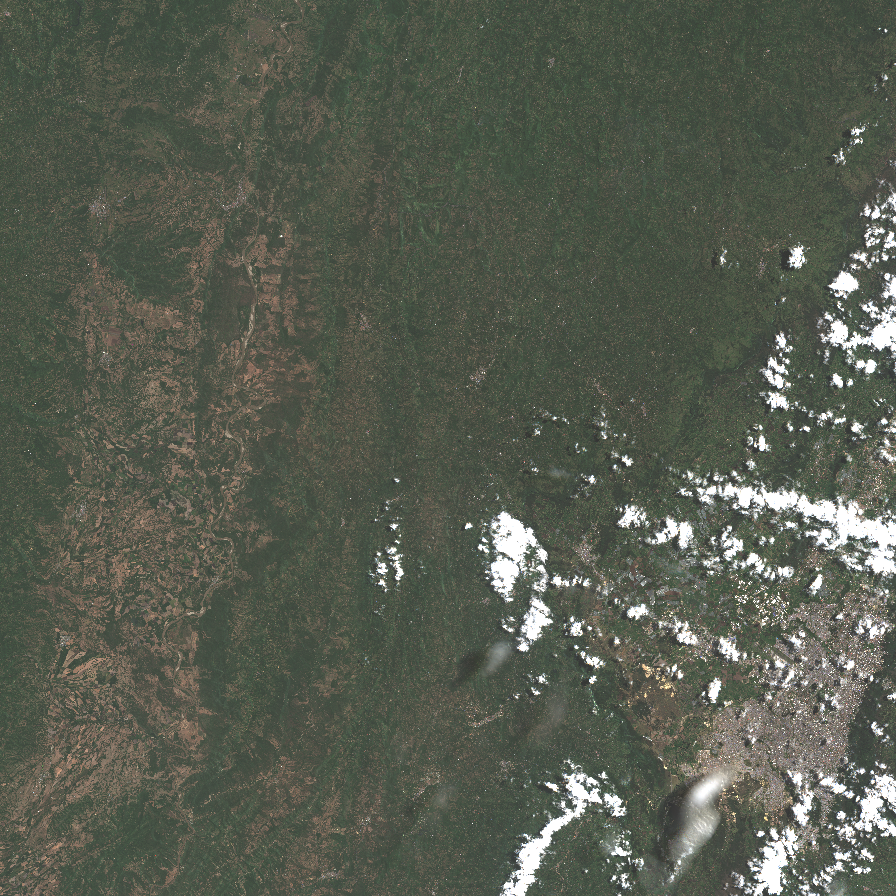
\includegraphics[width=0.85\textwidth]{stack_full.png}
\caption{Full Sentinel-2 scene (\texttt{armero\_stack.tif}) covering tile T18NWL before clipping to the ROI. True color composite (B4-B3-B2).}
\label{fig:stack}
\end{figure}

\subsection{Spectral Bands Used}

\begin{table}[H]
\centering
\begin{tabular}{|c|m{6cm}|c|}
\hline
\textbf{Band} & \textbf{Description} & \textbf{Native Resolution} \\
\hline
B2 & Blue & 10 m \\
\hline
B3 & Green & 10 m \\
\hline
B4 & Red & 10 m \\
\hline
B5 & Vegetation Red Edge 1 & 20 m (resampled to 10 m) \\
\hline
B6 & Vegetation Red Edge 2 & 20 m (resampled to 10 m) \\
\hline
B7 & Vegetation Red Edge 3 & 20 m (resampled to 10 m) \\
\hline
B8 & Near Infrared (NIR) & 10 m \\
\hline
B8A & Narrow Near Infrared & 20 m (resampled to 10 m) \\
\hline
B11 & Short Wave Infrared 1 (SWIR) & 20 m (resampled to 10 m) \\
\hline
B12 & Short Wave Infrared 2 (SWIR) & 20 m (resampled to 10 m) \\
\hline
\end{tabular}
\caption{Spectral bands included in the multi-band stack}
\end{table}

Bands at 20 m resolution (B5, B6, B7, B8A, B11, B12) were resampled to 10 m using bilinear interpolation via the \texttt{resample()} function from the \texttt{terra} package in R, ensuring spatial consistency across all bands.

%------------------------------------------------
\section{Dataset Creation Methodology}
%------------------------------------------------

The dataset creation process follows a supervised classification workflow based on multispectral data extraction from Sentinel-2 L2A imagery acquired over the Armero region.

\subsection{Methodology Overview}

\begin{enumerate}
    \item Download of Sentinel-2 Level-2A imagery from the Copernicus Browser (\url{https://browser.dataspace.copernicus.eu/}) for the Armero Guayabal region, selecting the August 15, 2024 scene with 15\% cloud coverage.
    \item Stacking of individual spectral bands (JP2 format) into a single multi-band GeoTIFF using the \texttt{terra} package in R. Bands at 20~m resolution (B5, B6, B7, B8A, B11, B12) were resampled to 10~m to match the native resolution of B2, B3, B4, and B8.
    \item Clipping of the multi-band stack to the ROI extent using QGIS (\textit{Raster $\rightarrow$ Extraction $\rightarrow$ Clip Raster by Extent}), generating the file \texttt{armero\_recortado.tif}.
    \item Digitization of training polygons in QGIS over the clipped image in true color composite (R:B4, G:B3, B:B2) with contrast stretch between 500 and 3,500 reflectance units, identifying four land cover classes: \textit{Vegetacion}, \textit{Cultivos}, \textit{Suelo\_desnudo}, and \textit{Zona\_urbana}.
    \item Extraction of pixel-level spectral values within training polygons using the \texttt{extract()} function from the \texttt{terra} package, including geographic coordinates ($x$, $y$).
    \item Balanced random sampling of 2,000 pixels per class (8,000 total) using the \texttt{dplyr} package (\texttt{slice\_sample()}), ensuring class balance and computational efficiency.
    \item Export of the final dataset in Tab-Separated Values (TSV) format as \texttt{training\_data.tsv}.
\end{enumerate}

\begin{figure}[H]
\centering

\includegraphics[width=0.85\textwidth]{satellite_image.png}
\caption{Clipped Sentinel-2 image (\texttt{armero\_recortado.tif}) in true color composite (B4-B3-B2) with contrast stretch between 500 and 3,500 reflectance units. Dark green areas correspond to dense vegetation; light brown areas correspond to bare soil and croplands; the white cluster at center is Armero Guayabal.}
\label{fig:satellite}
\end{figure}

\begin{figure}[H]
\centering

\includegraphics[width=0.85\textwidth]{training_polygons.png}
\caption{Training polygons digitized over the Armero study area, color-coded by land cover class (\textit{Vegetacion}, \textit{Cultivos}, \textit{Suelo\_desnudo}, \textit{Zona\_urbana}).}
\label{fig:polygons}
\end{figure}

\subsection{Land Cover Classes}

\begin{table}[H]
\centering
\begin{tabular}{|m{5cm}|c|c|}
\hline
\textbf{Class} & \textbf{Pixels Sampled} & \textbf{Percentage} \\
\hline
Vegetacion (Vegetation) & 2,000 & 25\% \\
\hline
Cultivos (Croplands) & 2,000 & 25\% \\
\hline
Suelo\_desnudo (Bare Soil) & 2,000 & 25\% \\
\hline
Zona\_urbana (Urban Area) & 2,000 & 25\% \\
\hline
\textbf{Total} & \textbf{8,000} & \textbf{100\%} \\
\hline
\end{tabular}
\caption{Pixel distribution per land cover class (balanced sampling)}
\end{table}

\noindent\textit{Note:} Water bodies were not included as a class due to the difficulty of reliably identifying narrow river channels at 10~m spatial resolution within the study area.

%------------------------------------------------
\section{Dataset Structure}
%------------------------------------------------

The generated TSV file \texttt{training\_data.tsv} contains 8,000 rows, each representing an individual pixel extracted from the training polygons. The dataset includes the following columns:

\begin{table}[H]
\centering
\begin{tabular}{|c|m{9cm}|}
\hline
\textbf{Column} & \textbf{Description} \\
\hline
x & Pixel easting coordinate in UTM Zone 18N (EPSG:32618) \\
\hline
y & Pixel northing coordinate in UTM Zone 18N (EPSG:32618) \\
\hline
B2 & Blue band surface reflectance (10 m) \\
\hline
B3 & Green band surface reflectance (10 m) \\
\hline
B4 & Red band surface reflectance (10 m) \\
\hline
B5 & Red Edge 1 surface reflectance (resampled to 10 m) \\
\hline
B6 & Red Edge 2 surface reflectance (resampled to 10 m) \\
\hline
B7 & Red Edge 3 surface reflectance (resampled to 10 m) \\
\hline
B8 & Near Infrared surface reflectance (10 m) \\
\hline
B8A & Narrow NIR surface reflectance (resampled to 10 m) \\
\hline
B11 & SWIR 1 surface reflectance (resampled to 10 m) \\
\hline
B12 & SWIR 2 surface reflectance (resampled to 10 m) \\
\hline
clase & Ground truth land cover label \\
\hline
\end{tabular}
\caption{Structure of the TSV training dataset}
\end{table}

%------------------------------------------------
\section{Expected Outcome}
%------------------------------------------------

The expected result of this first phase is the creation of a structured, balanced spectral dataset suitable for supervised machine learning training. This dataset will be used to evaluate five classification architectures:

\begin{itemize}
    \item Decision Trees (DT)
    \item Support Vector Machines (SVM)
    \item Artificial Neural Networks (ANN)
    \item K-Nearest Neighbor (KNN)
    \item Naive Bayes (NB)
\end{itemize}

Performance will be assessed using Confusion Matrix, Overall Accuracy, Kappa Coefficient, Precision, Recall, and F1-Score metrics.

%------------------------------------------------
\section{Conclusion}
%------------------------------------------------

This first phase establishes the conceptual and technical foundation of the project by defining the study area, selecting the satellite imagery, and designing the methodology for spectral data extraction. The generated dataset of 8,000 balanced pixels across four land cover classes will support future classification, validation, and thematic mapping tasks for the Armero region.

The use of Sentinel-2 L2A imagery with 15\% cloud coverage from August 15, 2024, combined with a balanced sampling strategy of 2,000 pixels per class, provides a robust and representative training set for the subsequent machine learning phases.

\end{document}